El algoritmo de solución ingenua es iterar sobre todos los pares de segmentos en $O(n^2)$ y verifique para cada par si se cruzan o no. Vamos a elaborar un algoritmo que sea mas eficiente que la solución ingenua basado en el \textbf{algoritmo de línea de barrido (\emph{sweep line})}.

Dibujemos una línea vertical $x = -\infty$ mentalmente y comience a mover esta línea hacia la derecha. En el curso de su movimiento, esta línea se encontrará con segmentos, y cada vez que un segmento se interseca con nuestra línea, se interseca exactamente en un punto (supondremos que no hay segmentos verticales).

% TODO: \usepackage{graphicx} required
\begin{figure}[h!]
	\centering
	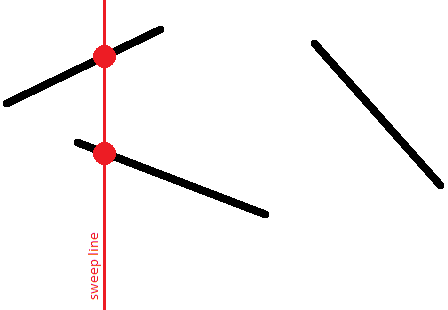
\includegraphics[width=0.3\linewidth]{img/sweep_line_1}
	\label{fig:sweepline1}
\end{figure}


Así, para cada segmento, en algún momento, su punto aparecerá en la línea de barrido, luego, con el movimiento de la línea, este punto se moverá y, finalmente, en algún momento, el segmento desaparecerá de la línea.

Estamos interesados en el \textbf{orden relativo de los segmentos} a lo largo de la vertical. Es decir, almacenaremos una lista de segmentos que cruzan la línea de barrido en un momento dado, donde los segmentos se ordenarán por su $y$-coordenada en la línea de barrido.

\begin{figure}[h!]
	\centering
	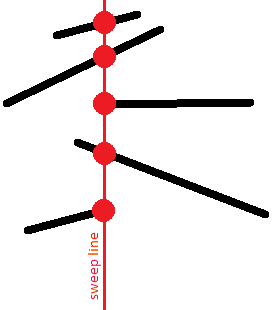
\includegraphics[width=0.2\linewidth]{img/sweep_line_2}
	\label{fig:sweepline2}
\end{figure}

Este orden es interesante porque los segmentos que se cruzan tendrán el mismo $y$-coordinar al menos en un momento:

\begin{figure}[h!]
	\centering
	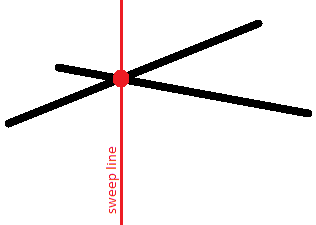
\includegraphics[width=0.3\linewidth]{img/sweep_line_3}
	\label{fig:sweepline3}
\end{figure}

Formulamos declaraciones clave:

\begin{itemize}
	\item Para encontrar un par que se interseque, es suficiente considerar \textbf{solo segmentos adyacentes} en cada posición fija de la línea de barrido.
	\item Basta con considerar la línea de barrido no en todas las posiciones reales posibles $(-\infty\ldots +\infty)$, pero \textbf{sólo en aquellas posiciones en las que aparecen nuevos segmentos o desaparecen los antiguos}. En otras palabras, es suficiente limitarse solo a las posiciones iguales a las abscisas de los puntos finales de los segmentos.
	\item Cuando aparece un nuevo segmento de línea, basta con \textbf{insertarlo} en la ubicación deseada en la lista obtenida para la línea de barrido anterior. Solo debemos verificar la intersección del \textbf{segmento agregado con sus vecinos inmediatos en la lista de arriba y abajo}.
	\item Si el segmento desaparece, basta con \textbf{eliminarlo} de la lista actual. Después de eso, es necesario \textbf{verificar la intersección de los vecinos superior e inferior en la lista}.
	\item No existen otros cambios en la secuencia de segmentos de la lista, excepto los descritos. No se requieren otros controles de intersección.
\end{itemize}

Para comprender la veracidad de estas afirmaciones bastan las siguientes observaciones:

\begin{enumerate}
	\item Dos segmentos disjuntos nunca cambian su orden relativo. De hecho, si un segmento fue primero más alto que el otro y luego se volvió más bajo, entonces entre estos dos momentos hubo una intersección de estos dos segmentos.
	\item Dos segmentos que no se intersecan tampoco pueden tener el mismo $y$-coordenadas.
	\item De esto se deduce que en el momento de la aparición del segmento podemos encontrar la posición de este segmento en la cola, y ya no tendremos que reorganizar este segmento en la cola: \textbf{su orden relativo a otros segmentos en la cola no cambiará}.
	\item Dos segmentos que se intersecan en el momento de su punto de intersección serán vecinos entre sí en la cola.
	\item Por lo tanto, para encontrar pares de segmentos de línea que se intersecan, es suficiente verificar la intersección de todos y solo aquellos pares de segmentos que en algún momento durante el movimiento de la línea de barrido al menos una vez fueron vecinos entre sí. 
	
	Es fácil notar que solo basta con verificar el segmento agregado con sus vecinos superior e inferior, así como al eliminar el segmento, sus vecinos superior e inferior (que después de la eliminación se convertirán en vecinos entre sí).
	\item Cabe señalar que en una posición fija de la línea de barrido, primero debemos \textbf{agregar todos los segmentos} que comienzan en esta coordenada x, y solo \textbf{luego eliminar todos los segmentos} que terminan aquí. 
	
	Por lo tanto, no perdemos la intersección de los segmentos en el vértice: es decir, los casos en que dos segmentos tienen un vértice común.
	
	\item Tenga en cuenta que \textbf{los segmentos verticales} en realidad no afectan la corrección del algoritmo.
	Estos segmentos se distinguen por el hecho de que aparecen y desaparecen al mismo tiempo. Sin embargo, debido al comentario anterior, sabemos que todos los segmentos se agregarán primero a la cola y solo luego se eliminarán. Por lo tanto, si el segmento vertical se cruza con algún otro segmento abierto en ese momento (incluido el vertical), será detectado.
	\textbf{¿En qué lugar de la cola colocar los segmentos verticales?} Después de todo, un segmento vertical no tiene un segmento específico. $y$-coordenada, se extiende por todo un segmento a lo largo de la $y$-coordinar. Sin embargo, es fácil entender que cualquier coordenada de este segmento puede tomarse como $y$-coordinar.
\end{enumerate}
